\section*{Manuales de usuario} \label{sec:ManualesdeUsuario}
\addcontentsline{toc}{section}{Manuales de usuario}

\begin{multicols}{2} 
\subsection*{Consultas a base de datos}

Existen dos tipos de consultas básicas: consultas por zona determinada o por rango de frecuencia. Usted puede elegir consultar a nivel nacional, en una entidad territorial, departamento o municipio. Las consultas requieren un poco de tiempo en desplegarse debido a que presentan información considerable, considere usar una conexión de al menos 516 kbps.

\begin{figure}[H]
	\centering
	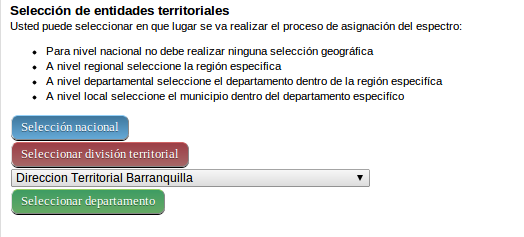
\includegraphics[width=8.5cm]{Anexos/Imagenes/ManualUsuario/ConsultasGeografica.png}
	\caption{Filtro en la consulta por zona geográfica.}
\end{figure}

Usted puede elegir la zona geográfica que desea consultar.
	
\begin{figure}[H]
	\centering
	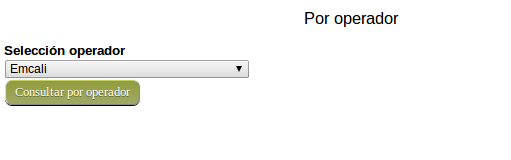
\includegraphics[width=6.5cm]{Anexos/Imagenes/ManualUsuario/FiltroPorOperador.png}
	\caption{Filtro en la consulta por operador.}
\end{figure}

En esta pantalla usted puede elegir el operador al cual se va consultar su asignación.

\begin{figure}[H]
	\centering
	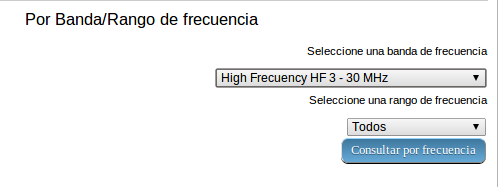
\includegraphics[width=6.5cm]{Anexos/Imagenes/ManualUsuario/FiltroPorBanda.png}
	\caption{Filtro en la consulta por banda.}
\end{figure}

En esta consulta se puede elegir la banda que se desea consultar.

\subsection*{Gestión Operadores}

Estas operaciones sólo las puede realizar un usuario con rol administrador de espectro.

\begin{figure}[H]
	\centering
	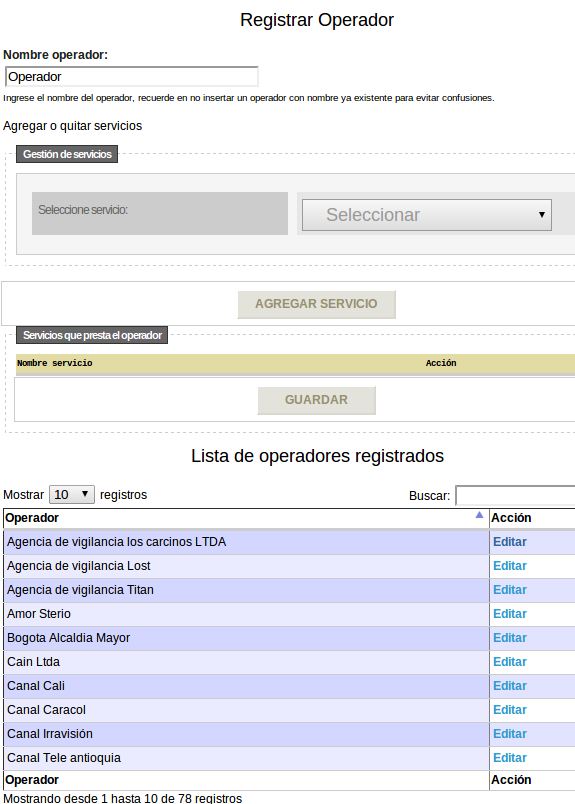
\includegraphics[width=6.5cm]{Anexos/Imagenes/ManualUsuario/Operador.png}
	\caption{Registrar operador}
\end{figure}

Para registrar un operador, usted debe definir sus parámetros y hacer clic en guardar.
	

\begin{figure}[H]
	\centering
	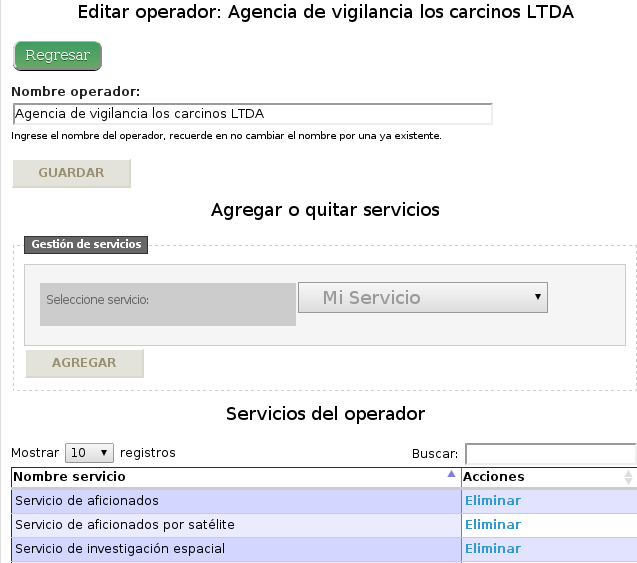
\includegraphics[width=6cm]{Anexos/Imagenes/ManualUsuario/OperadorEditar.png}
	\caption{Editar operador.}
\end{figure}

Para editar un operador, puede editar cualquier de los cambios y servicios asociados a el.
	
\subsection*{Gestión Servicios.}

Estas operaciones sólo las puede realizar un usuario con rol administrador de espectro.


\begin{figure}[H]
	\centering
	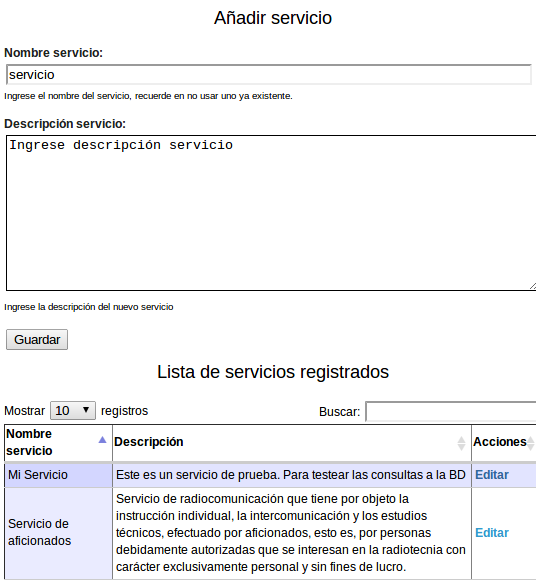
\includegraphics[width=5cm]{Anexos/Imagenes/ManualUsuario/Servicios.png}
	\caption{Agregar servicio.}
\end{figure}

Para agregar un servicio, se debe definir un nombre y su descripción, finalmente hacer clic en guardar.	
	
\begin{figure}[H]
	\centering
	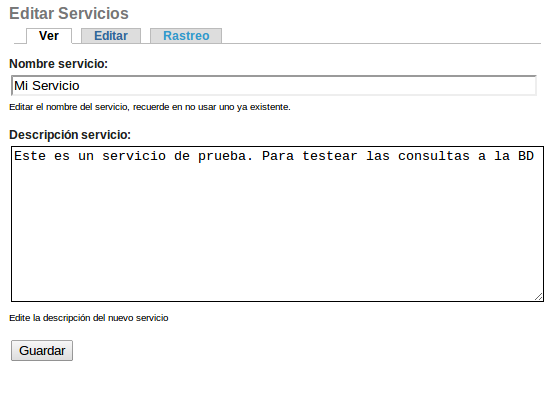
\includegraphics[width=6.5cm]{Anexos/Imagenes/ManualUsuario/EditarServicios.png}
	\caption{Editar servicio.}
\end{figure}

Aquí usted podrá editar los parámetros asociados de un servicio.
	
\subsection*{Gestión Rangos de Frecuencia}

Estas operaciones sólo las puede realizar un usuario con rol administrador de espectro.

\begin{figure}[H]
	\centering
	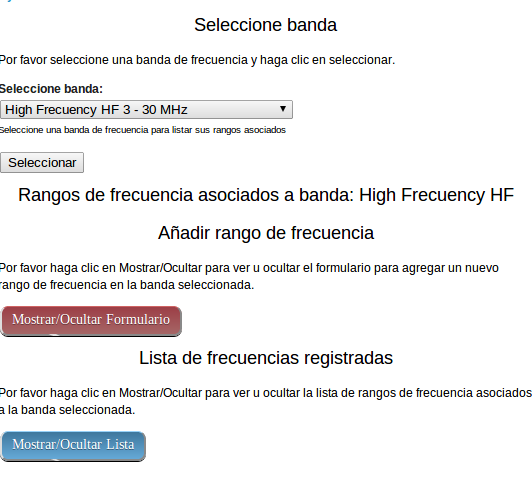
\includegraphics[width=6cm]{Anexos/Imagenes/ManualUsuario/SeleccionBanda.png}
	\caption{ Selección banda de frecuencia.}
\end{figure}

En esta pantalla usted podrá seleccionar la banda de frecuencia para realizar acciones sobre los rangos de frecuencia asociados a ella.

\begin{figure}[H]
	\centering
	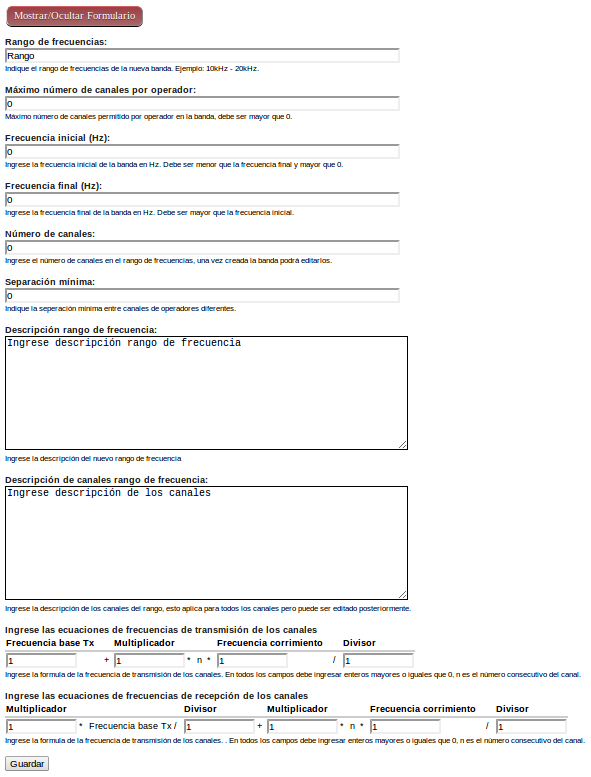
\includegraphics[width=7cm]{Anexos/Imagenes/ManualUsuario/AgregarRangoFrecuencia.png}
	\caption{ Agregar banda de frecuencia.}
\end{figure}

En este campo usted podrá crear un nuevo rango de frecuencia, especificando cada uno de los datos del rango y las formulas que se aplican para el cálculo de las frecuencias de transmisión y recepción de cada uno de los canales del nuevo rango de frecuencia.

\begin{figure}[H]
	\centering
	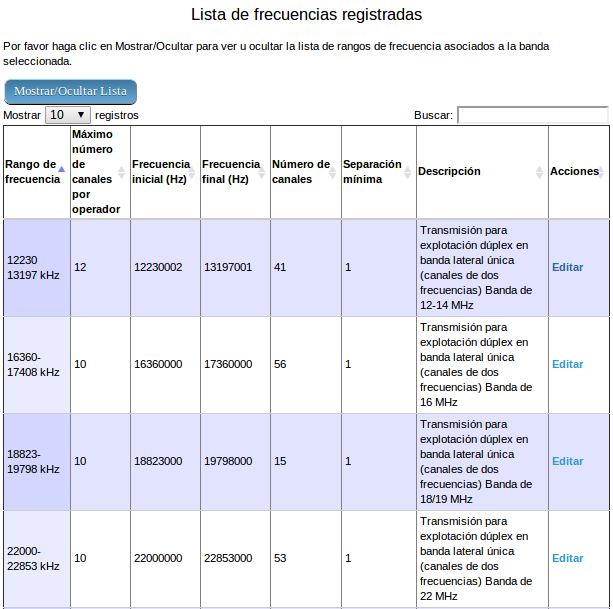
\includegraphics[width=6.5cm]{Anexos/Imagenes/ManualUsuario/FrecuenciasRegistradas.png}
	\caption{ Lista de rangos de frecuencia registrados en una banda.}
\end{figure}

En esta pantalla, usted podrá elegir que rango de frecuencia desea editar.

\begin{figure}[H]
	\centering
	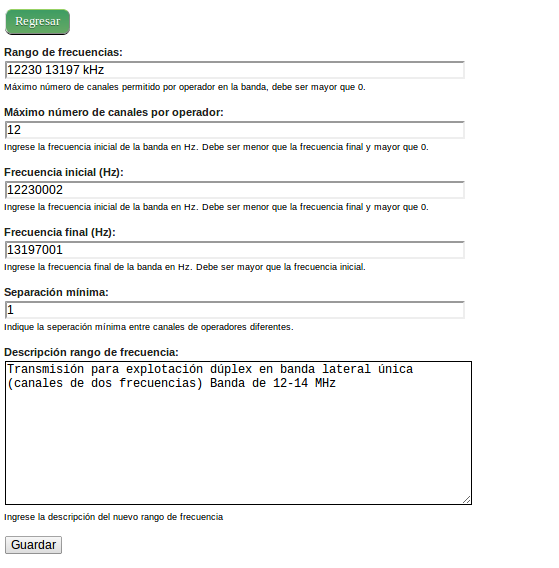
\includegraphics[width=5cm]{Anexos/Imagenes/ManualUsuario/EditarRangoFrecuencia.png}
	\caption{ Editar rango de frecuencia.}
\end{figure}

La operación editar rango de frecuencia permite editar los parámetros asociados a un rango de frecuencia.

\begin{figure}[H]
	\centering
	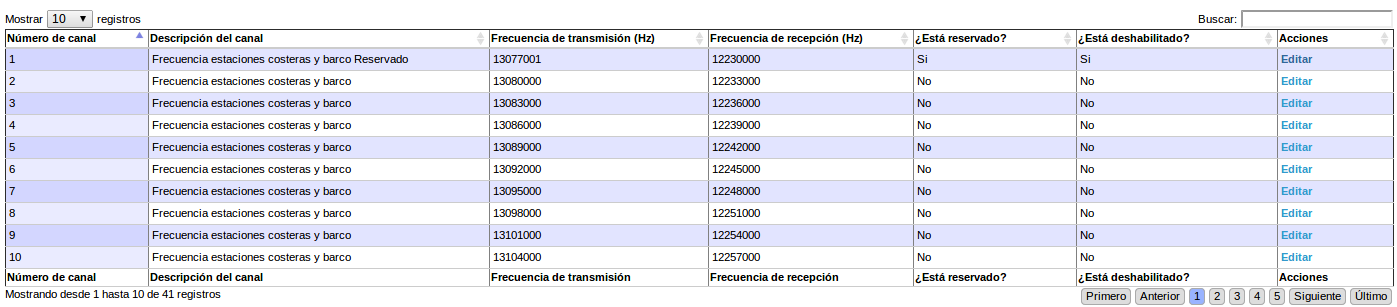
\includegraphics[width=8cm]{Anexos/Imagenes/ManualUsuario/Canales.png}
	\caption{ Lista de canales asociados a un rango de frecuencia.}
\end{figure}

Es la lista de canales asociados a un rango de frecuencia, si usted desea editar alguno de ellos debe hacer clic en \textit{Editar}.

\begin{figure}[H]
	\centering
	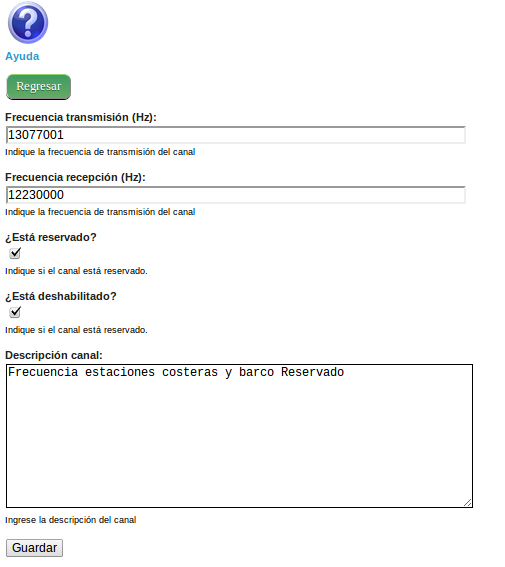
\includegraphics[width=5cm]{Anexos/Imagenes/ManualUsuario/EditarCanal.png}
	\caption{ Editar canal.}
\end{figure}

Al hacer clic en editar, usted puede editar los parámetros asociados a un canal de un rango de frecuencia.

\subsection*{Gestión Entradas XML}

\begin{figure}[H]
	\centering
	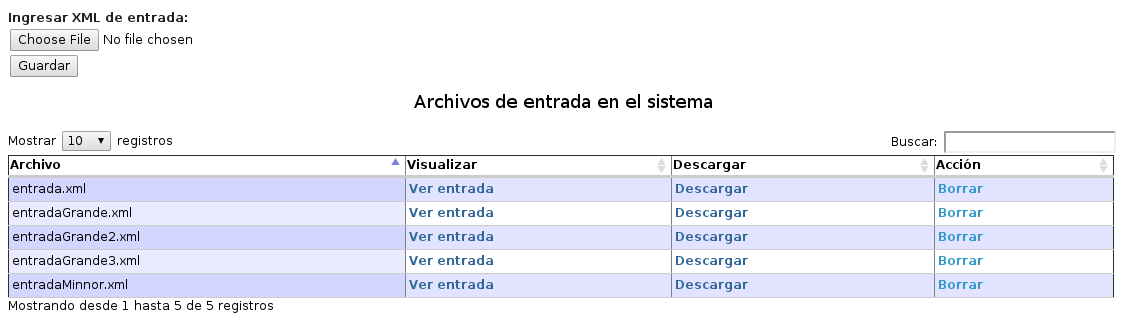
\includegraphics[width=7.5cm]{Anexos/Imagenes/ManualUsuario/Entradas.png}
	\caption{ Lista de entradas XML almacenadas en el sistema.}
\end{figure}

La gestión de entradas XML permite visualizar, descargar y borrar las entradas XML propias de un usuario.

\subsection*{Gestión Salidas XML}

\begin{figure}[H]
	\centering
	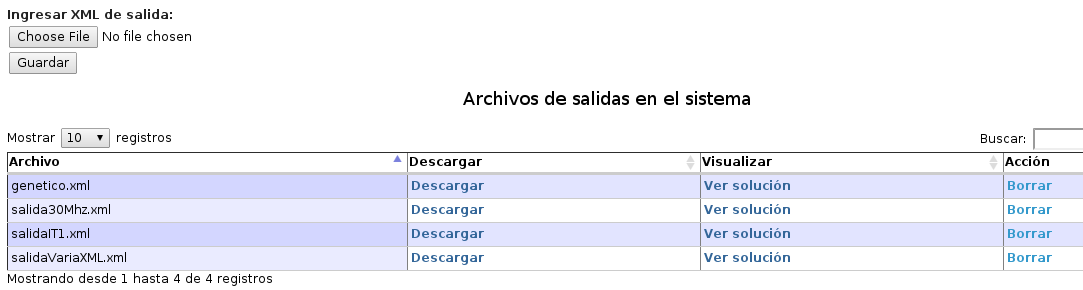
\includegraphics[width=7.5cm]{Anexos/Imagenes/ManualUsuario/Salidas.png}
	\caption{ Lista de salidas XML almacenadas en el sistema.}
\end{figure}

La gestión de salidas XML permite visualizar, descargar y borrar las salidas XML propias de un usuario.

\subsection*{Generador de entradas}

En el generador de entradas, usted debe seleccionar la zona geográfica y la banda de frecuencia en donde desea realizar un requerimiento, una vez hecho éste proceso puede proceder a crear los requerimientos de la entrada.

\begin{figure}[H]
	\centering
	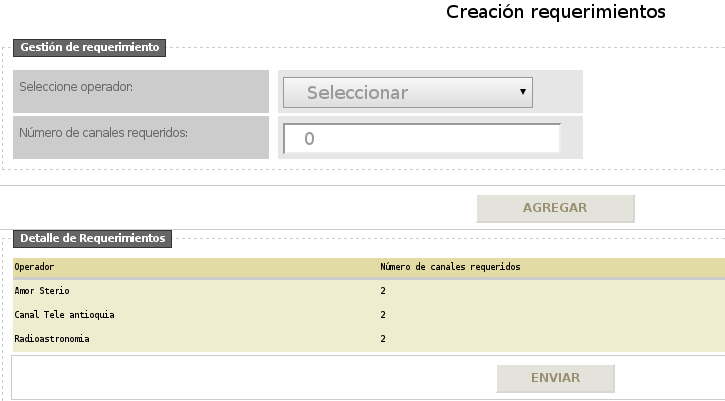
\includegraphics[width=5cm]{Anexos/Imagenes/ManualUsuario/Requerimientos.png}
	\caption{ Especificación de requerimientos.}
\end{figure}

Una vez haga la creación de requerimientos podrá generar la entrada XML y almacenarla en el sistema.

\subsection*{Actualizar Base de datos}

Estas operaciones sólo las puede realizar un usuario con rol administrador de espectro.

\begin{figure}[H]
	\centering
	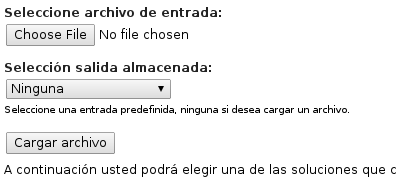
\includegraphics[width=6.5cm]{Anexos/Imagenes/ManualUsuario/Entrada.png}
	\caption{ Selección salida XML para actualizar base de datos.}
\end{figure}

Usted debe seleccionar un archivo de salida o ingresar uno, para registrar su información a la base de datos.

\begin{figure}[H]
	\centering
	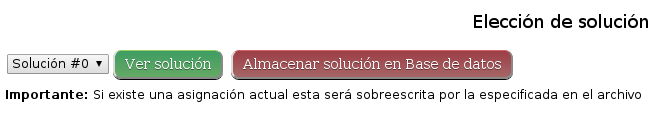
\includegraphics[width=6.5cm]{Anexos/Imagenes/ManualUsuario/ElegirSolucion.png}
	\caption{ Selección entrada XML para actualizar base de datos.}
\end{figure}

Es importante aclarar que una asignación con datos incorrectos, puede comprometer la integridad de los datos de la base de datos.

\subsection*{Aplicativos} \label{manual:aplicativo}

Existen dos aplicativos en el proyecto, por programación por restricciones y por algoritmo genético. 

\begin{figure}[H]
	\centering
	\label{fig:appCPP}
	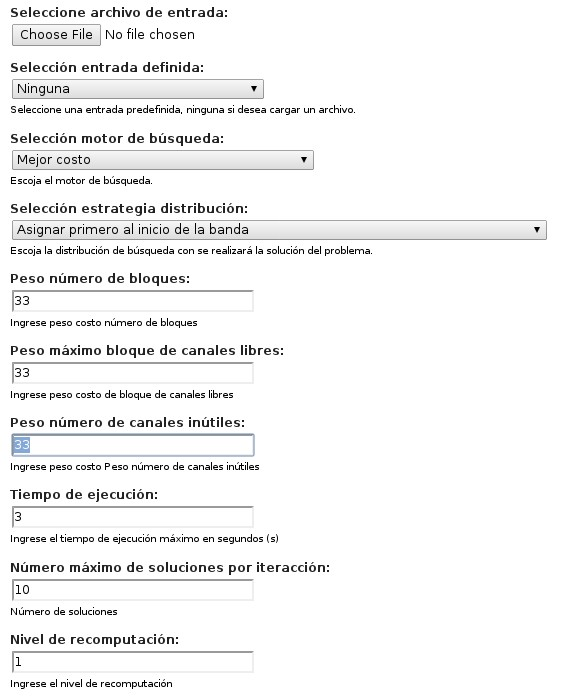
\includegraphics[width=7.5cm]{Anexos/Imagenes/ManualUsuario/Aplicacion.jpeg}
	\caption{ Aplicativo por programación por restricciones.}
\end{figure}

\begin{figure}[H]
	\centering
	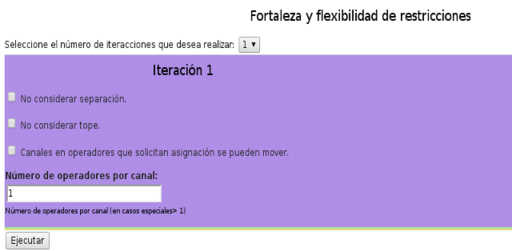
\includegraphics[width=6cm]{Anexos/Imagenes/ManualUsuario/Flexibilidad.png}
	\caption{ Flexibilidad y debilidad de restricciones.}
\end{figure}

En la flexibilidad se pueden dfinir que restricciones no se toman en cuenta y decidir cuantas iteraciones se van a realizar.

\begin{figure}[H]
	\centering
	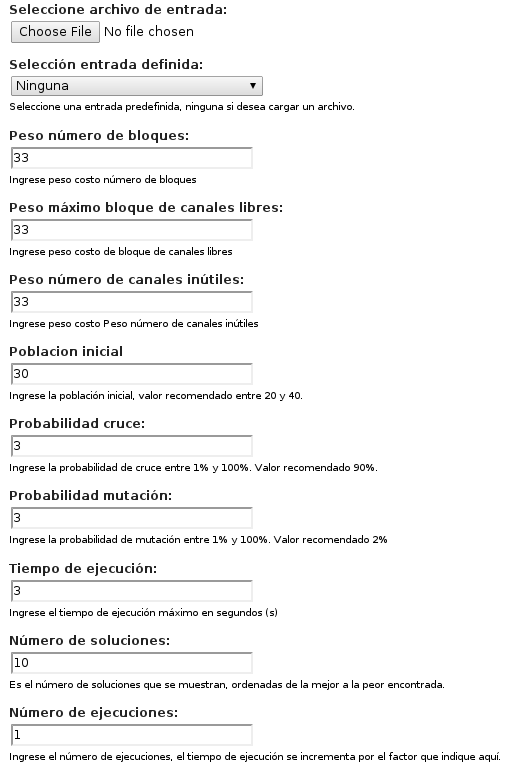
\includegraphics[width=7.5cm]{Anexos/Imagenes/ManualUsuario/genetico.png}
	\caption{ Aplicativo por algortimo genético.}
\end{figure}

Los resultados se despliegan mostrando la información general de la ejecución, un listado de soluciones encontradas y el detalle de que cada solución.

\begin{figure}[H]
	\centering
	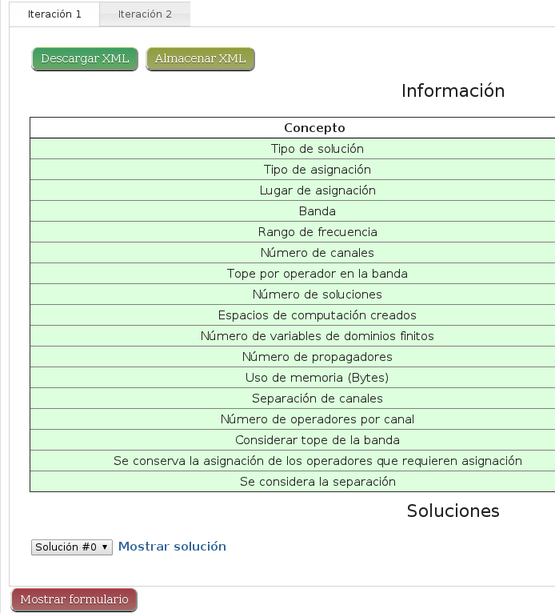
\includegraphics[width=7.5cm]{Anexos/Imagenes/ManualUsuario/Resultados.png}
	\caption{ Información general acerca de una salida XML.}
\end{figure}

\end{multicols} 

\begin{figure}[H]
	\centering
	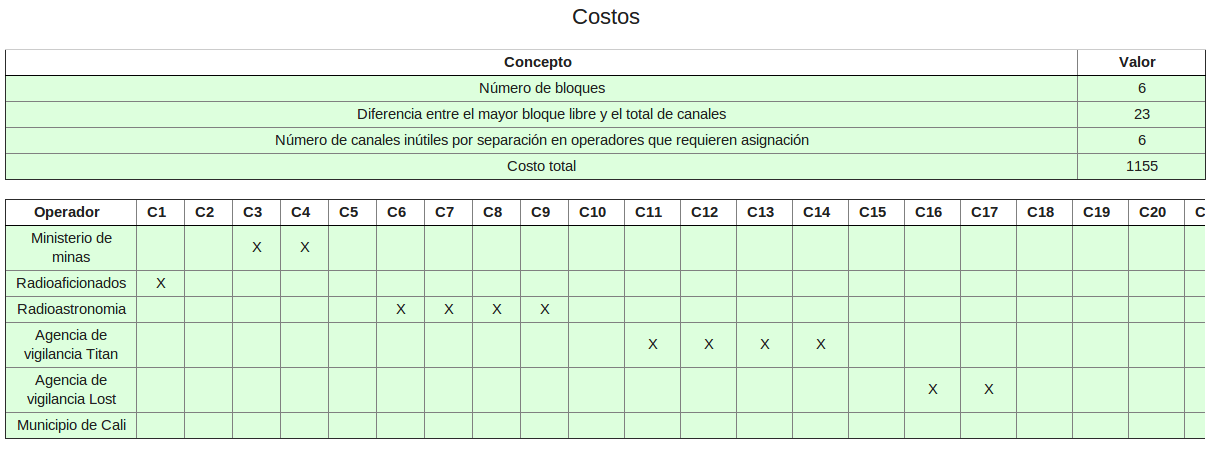
\includegraphics[width=15cm]{Anexos/Imagenes/ManualUsuario/ResultadosCostos.png}
	\caption{ Información de costos y reporte de una solución obtenida de una salida XML.}
\end{figure}




